\chapter{Dual-Branch Structuring of the Latent Space for Disentangling and Image Editing}
\label{chapter:dualdis}

\renewcommand{\leftmark}{\spacedlowsmallcaps{Structuring the Latent Space for Disentangling and Image Editing}}

\begin{chapabstract}
    {\em
    
    To complete our work on latent representations of images, we address the problem of producing disentangled latent representations, which means finding representations that model individual factors of variation in the data.
    For this, we propose DualDis, a new auto-encoder-based framework that separates and linearizes two complementary types of information that we call class and attributes, improving the semantic quality of the representations and their complementarity. This is achieved thanks to a two-branch architecture forcing the separation of the two kinds of information, accompanied by a decoder for image reconstruction and generation. To effectively separate the information, we propose to use a combination of regular and adversarial classifiers to guide the two branches in specializing for class and attribute information respectively. We also investigate the possibility of using semi-supervised learning for an effective disentangling even using few labels. We leverage the linearization property of the latent spaces for semantic image editing and generation of new images. We validate our approach on CelebA, Yale-B and NORB by measuring the efficiency of information separation via classification metrics, visual image manipulation and data augmentation.

    \vspace*{5mm}
    The work in this chapter has led to the submission of a conference paper currently under review:}
    \begin{itemize}
        \item \small \fullcite{Robert2019}.
    \end{itemize}
\end{chapabstract}

\ifthenelse{\boolean{skipDual}}{\endinput}{}


\newpage

\minitoc
\chapterwithfigures{\nameref*{chapter:dualdis}}
\chapterwithtables{\nameref*{chapter:dualdis}}

\section{Introduction}

In the previous chapter, we proposed to separate the visual information contained in an image in two latent spaces, one for the discriminative information related to the category, and one for the non-discriminative information. This was done in order to improve the accuracy of a classifier in the context of \ac{SSL} by solving a conflict between two popular ways of regularizing \acp{DNN} using HybridNet. One interpretation of the behavior of HybridNet is that its first branch encodes discriminative information that is related to the general pattern of the image (related to the class) while the second and complementary unsupervised branch focuses on details independent of the class such as local textures, detailed shape, \etc.

In this chapter, we propose to pursue further this interpretation of information separation and tackle the problem of \textit{disentangling}.
In \ac{DL} and especially in the \ac{CV} community, this problem of disentangling factors of variation is a very active field of research, \textit{cf.} \citet{higgins2018towards}. The exact objective of those model vary but the overall idea of disentangling is to increase the quality of the latent representations so that they represent independent factors of variation in the data. We will see that this can be done in various ways.

By improving the semantic quality of the representations and their independence, disentangling can be used to improve many applications such as transfer learning \citep{ruiz2019learning}, domain adaptation \citep{chang2019all,louizos2016}, information retrieval \citep{Mathieu2016}, image generation \citep{perarnau2016invertible}, \etc. In addition, since these models are usually based on encoder-decoder architectures, they can combine \textit{visual understanding} and \textit{image generation}. For the particular application of image generation, while disentangling models do not yet compete with powerful generative models \citep[\eg\unskip][]{karras2018style} regarding the quality of generated images, they are an interesting direction for controlling latent conditional factors regarding what is being generated, which remains a challenging task in this literature.


To address this problem, we propose to further explore structured latent representations of images, in continuation of our work in \autoref{chapter:hybridnet}, but this time designed for both \textit{image classification} and \textit{visual attribute detection}. We are interested in modeling two complementary kinds of information that we will call \textit{information domains}. For example, with a face dataset, we would like to represent the identity (\ie the class) of the person and various visual attributes (hairstyle, makeup, facial expression, \etc.). This direction thus addresses the question of producing complementary representation spaces that improve their cooperation to structure the information, generalize better and produce good reconstructions and generations.

\begin{figure}[p]
    \begin{subfigure}[t]{\linewidth}
        \centering
        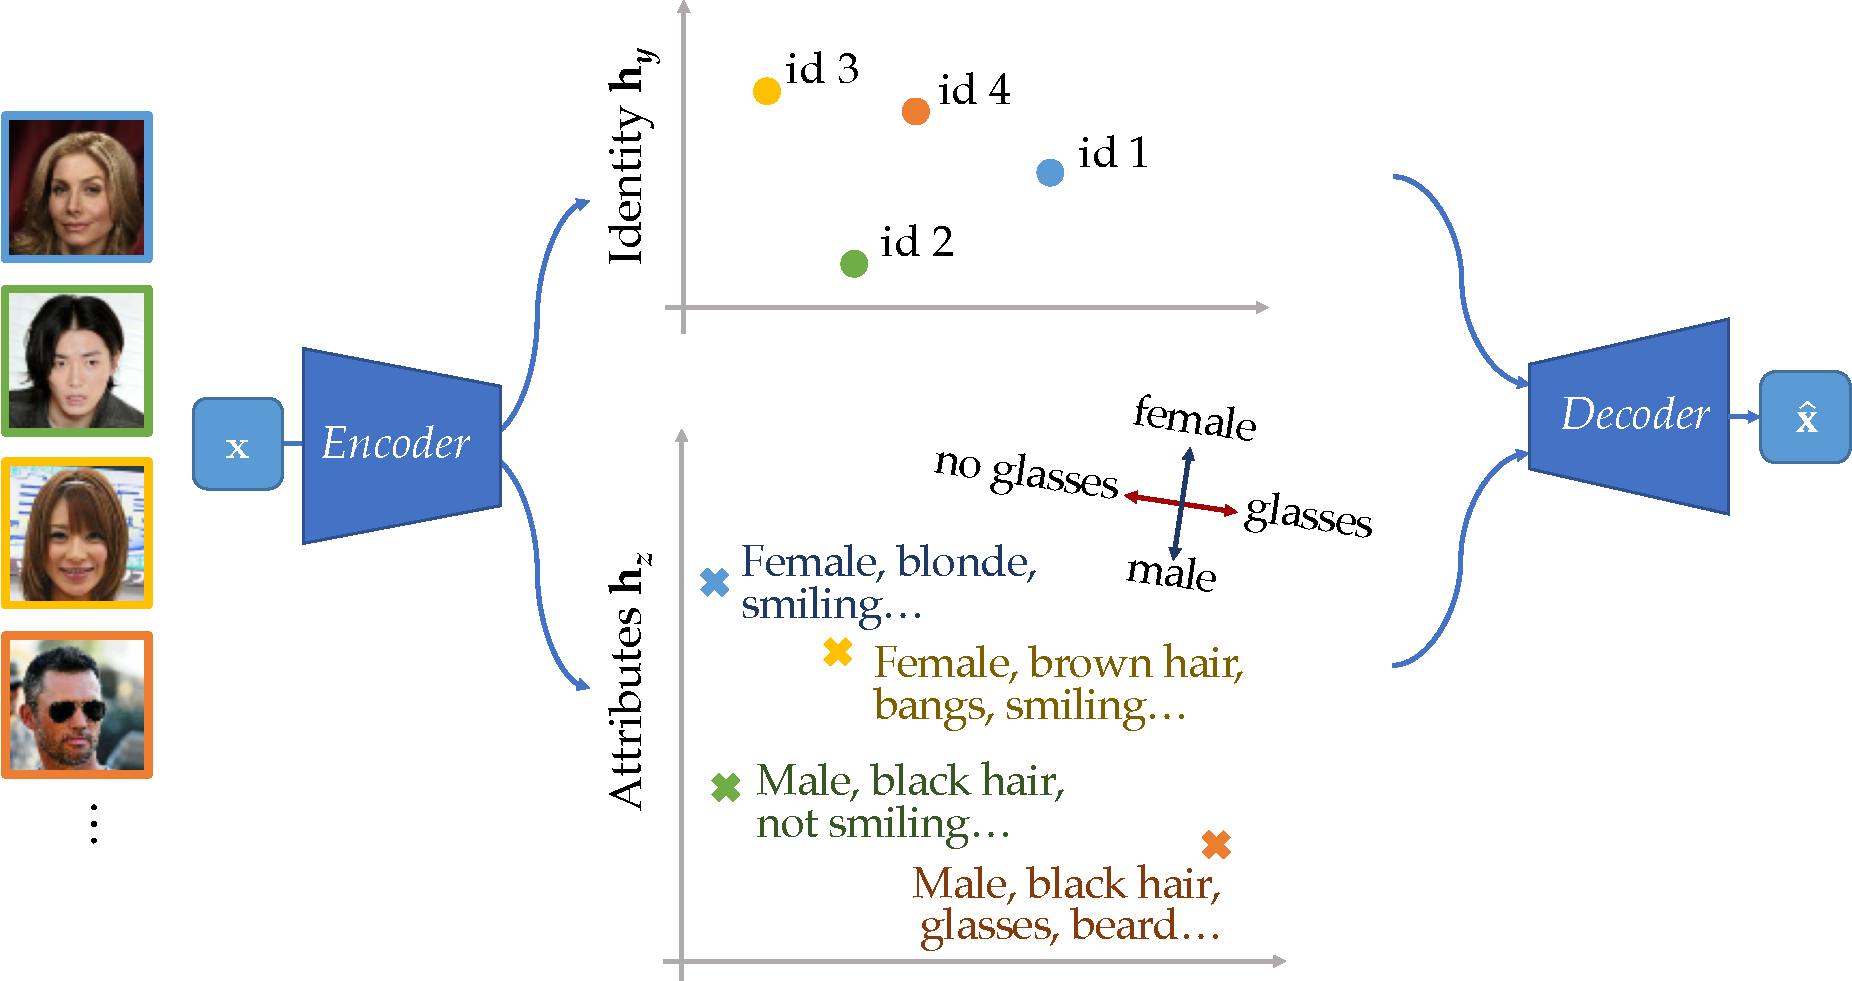
\includegraphics[width=\linewidth]{images/dualdis_intro_1}\\[0.3em]
        \titlecaption[c]{Behavior of our encoder-decoder}{\unskip, learned to explicitly separate complementary representations of identity (top) and attributes (bottom) in dual latent subspaces.}
        \label{dualdis:fig:motivation:a}
    \end{subfigure}
    
    \begin{subfigure}[t]{\linewidth}
        \centering
        \vspace{1.2em}
        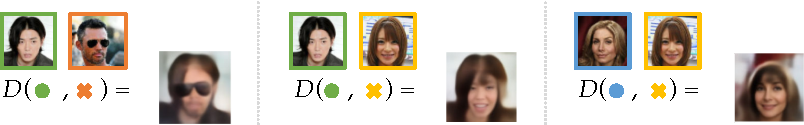
\includegraphics[width=\linewidth]{images/dualdis_intro_2}\\[0.3em]
        \titlecaption[c]{Illustration of the \textit{disentangling} ability of DualDis}{\unskip, mixing the identity of a first image and the attributes of a second. In the middle example, the man framed in green takes the attributes of the women framed in yellow, becoming a smiling woman with brown bangs.}
        \label{dualdis:fig:motivation:b}
    \end{subfigure}
    
    \begin{subfigure}[t]{\linewidth}
        \centering
        \vspace{1.2em}
        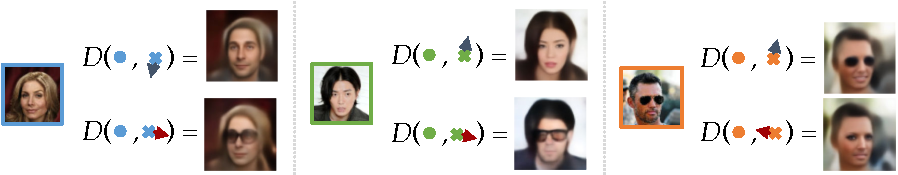
\includegraphics[width=\linewidth]{images/dualdis_intro_3}\\[0.3em]
        \titlecaption[c]{Illustration of the \textit{image editing} ability of DualDis}{\unskip, provided by the linearization of the factors of variation. For the first example (woman framed in blue), we move the representation \textcolor{bluefig}{\scriptsize \ding{54}} along the directions male (first line) and glasses (second line) to add those attributes.}
        \label{dualdis:fig:motivation:c}
    \end{subfigure}
    
    \titlecaption{Overview of our DualDis framework}{We present the general behavior of the model (a) and illustrate its abilities at disentangling (b) and editing images (c).}
    \label{dualdis:fig:motivation}
\end{figure}

While HybridNet focused on separating discriminative and non-discriminative information, with a clear asymmetry between the two, here we separate two similarly interesting types of information. 
Leveraging the insights of the previous chapter, we propose \textbf{DualDis}, a dual-branch deep \ac{AE} that explicitly separates the information domains in two distinct latent subspaces as schematized in \autoref{dualdis:fig:motivation:a}: one space $\vhy$ for class-related information and other $\vhz$ for attribute-related information. A decoder $D(\vhy, \vhz)$ is then used to reconstruct images and generate new ones.
%
An important contribution lies in the learning strategy that we propose.
Using adversarial training, we are able to explicitly find and remove wrongly organized information and effectively separate and ``orthogonalize'' the two information domains. This disentangling behavior is illustrated in \autoref{dualdis:fig:motivation:b} where we show that it allows mixing representations of different images.

In addition, our architecture is also designed to linearize the factors of variation in each latent space.
This reinforces the semantic quality of the representations and means that simple linear shifts of a latent representation in given directions are directly linked to known semantic factors.
Taking advantage of this property, we can perform image editing by modifying the representations of a given image. This is illustrated in \autoref{dualdis:fig:motivation:c}, where we change the gender and eyeglasses attributes of images while conserving the identity and the other attributes. This is done by following the linear directions provided by the model, as shown on the left of the figure. Thanks to this, we can also perform \textit{guided} \acf{DA} by generating variations of images with semantic changes instead of low-level changes (flip, translation, color jitter, \textit{etc.}) as usually done.

In this chapter, we first present the state of the art in \autoref{dualdis:sec:RW}, then we present DualDis in depth in \autoref{dualdis:sec:model} and we validate the effectiveness of our approach in the next sections quantitatively (\autoref{dualdis:sec:exp}), using \ac{SSL} (\autoref{dualdis:sec:ssl}), and for editing (\autoref{dualdis:sec:editing}).

\section{Related work} \label{dualdis:sec:RW}

In this chapter, we try to go one step closer to eventually ``bridging the gap'' between discriminative and generative models. Indeed, our objective is to produce a model that both represents highly semantic information and is able to generate new data. We thus propose to go over some generative and disentangling models that exist in the literature.

\paragraph{Notations.} Because the standard notations vary from one domain to another, and to avoid any misunderstanding, we choose to unify the notations and use the ones that follow:
\begin{itemize}[leftmargin=2em]
    \item[$\vy,\vz$] Labels of the primary and secondary semantic information are designated respectively with $\vy$ and $\vz$. The primary information ($\vy$) corresponds to the class or identity of the subject of the image, while the secondary information $\vz$ corresponds to general visual attributes (\eg for faces it represent the expression, hairstyle, \etc).
    \item[$\vh$] All latent vectors are designed with $\vh$, including inputs of generative models.
    \item[$\tilde{\textcolor{lightgray}{\boxempty}}$] Vectors with a tilde correspond to elements that were randomly drawn from a prior distribution or generated from one (\eg $\vht\sim p(\vh), \vxt = G(\vht)$)
    \item[$\hat{\textcolor{lightgray}{\boxempty}}$] Vectors with a hat correspond to elements that are estimated and usually correspond to a known value (\eg $\vxh=D(E(\vx))$ is the reconstruction of a known input image $\vx$, $\vyh$ is a prediction of a ground truth $\vy$)
\end{itemize}

\FloatBarrier

\subsection{Generative models}

\begin{figure}[tb]
    \centering
    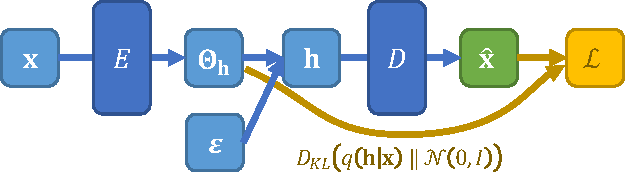
\includegraphics[width=0.6\textwidth]{images/dualdis_vae}\\
    ~\\
    ~\\
    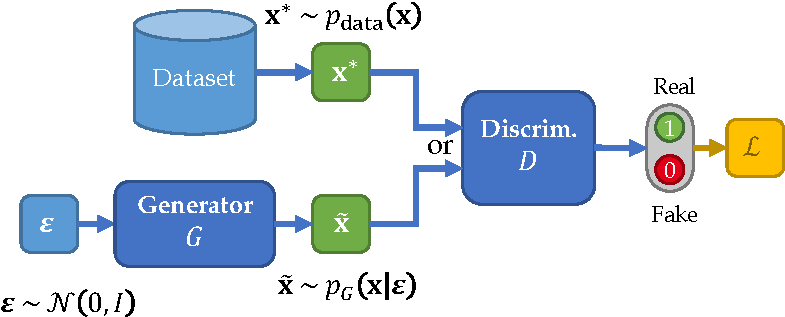
\includegraphics[width=0.74\textwidth]{images/dualdis_gan}
    \caption[Schematic representation of \acs{VAE} and \acs{GAN}]{Schematic representation of a \acs{VAE} (top) and a \acs{GAN} (bottom).}
    \label{dualdis:fig:vae_gan}
\end{figure}

First, we propose a quick overview of some modern generative models and how they represent the information.
In this context, the term \textit{generative models} refers to models that are able to generate new images $\vxt$ from a randomly sampled input noted $\vht$. In the recent \acf{DL} literature, there are two main types of models for this, \acfp{VAE} and \acfp{GAN}.

\paragraph{\acl{VAE}.} \acp{VAE} were introduced by \citet{Kingma2013} and can be seen as an extension of an \ac{AE}, represented in \autoref{dualdis:fig:vae_gan} (top). To summarize, after some modeling assumptions and lower-bounds of the data likelihood maximization $\max \log p(\vx)$, the training loss ends up consisting in adding a regularization term on the latent representations $\vh$ of an \ac{AE} so that they match a prior distribution $p_\mathrm{prior}(\vh)$:
\begin{equation}
    \mcL(\vx) = \mcL_\mathrm{rec} \big(\vx, \vxh \big) + \mcD_\mathrm{KL}\big( \vh\,||\,p_\mathrm{prior}(\vh) \big)
\end{equation}
During the training, the model does not generate samples, it simply learns to reconstruct and make sure that the representations $\vh$ respect the prior distribution. However, thanks to this prior distribution $p_\mathrm{prior}(\vh)$, after the training, it is possible to sample values $\vht\sim p(\vh)$ and use the decoder $D$ of the \ac{VAE} to obtain a new image $\vxt=D(\vht)$ that should belong to the distribution of real images. As we mentioned, this is ensured through the maximization of the data likelihood.

\paragraph{\acl{GAN}.} \acp{GAN} were proposed by \citet{Goodfellow2014} and rely on a different and original approach that directly addresses the question of producing realistic images, as represented in \autoref{dualdis:fig:vae_gan} (bottom). They propose to use a generator $G$ transforming an input noise $\vht \sim p_\mathrm{prior}(\vh)$ (with a chosen fixed prior $p_\mathrm{prior}(\vh)$) into an image $\vxt$. This generator is accompanied by a discriminator $D$ that learns to detect if its input $\vx$ is a real image from the dataset ($\vx^*$) or a generated image from $G$ ($\vxt$). The discriminator is trained to make correct predictions; and the generator is trained to fool the discriminator, \ie to produce images $\vxt$ that $D$ classify as real images. They have therefore opposite goals and are often said to be trained toward a Nash equilibrium.
\begin{equation}
    \vxt = G(\vht),\ \vht\sim p_\mathrm{prior}(\vh), \quad
    D(\vx) \in [0,1],\ \text{ideally, } \begin{cases}
    D(\tilde \vx) = 0, & \tilde \vx = G(\vht)\\
    D(\vx^*) = 1, & \vx^* \in \mcD_\mathrm{real}
\end{cases}
\end{equation}

Because of their particular training, the exact behavior of \acp{GAN} has been widely discussed. Very unstable especially in its early stages, solutions were proposed \citep{kodali2017convergence,roth2017stabilizing} and \acp{GAN} can now produce very high-quality images \citep{karras2017progressive,karras2018style} and can also be used for image-to-image translations (\eg changing maps into satellite images) \citep{zhu2017unpaired,choi2018stargan}, super-resolution \citep{ledig2017photo}, \etc.

A difference that is often discussed between \acp{GAN} and \acp{VAE} is the ``sharpness'' of the images produced. This phenomenon is studied and quantified more thoroughly by \citet{blau2018perception} in the context of super-resolution or image restoration and is described as the perception-distortion tradeoff. This shows that models that produce ``sharp'' looking images (\ie with good perceptual quality) are actually adding incorrect local information that does not correspond to the reality. Doing so, they actually produce more distortion (\ie difference with the ground truth) than models that produce blurry images. This may or may not be problematic depending on the application, \ie if matching a specific \textit{ground truth} is relevant or if artificial details are welcome.

\paragraph{Information representation in generative models.} 

First, we can note that unlike \acp{VAE} that come with an encoding model, \ac{GAN}-based models usually do not, making it impossible to know the representation $\vh$ of an existing image, which limits the possible applications to pure generation. To solve this, models propose variations of the original \ac{GAN} framework. They introduce an encoder $E(\vx)$ producing representations $\vh$ that the generator $G(\vh)$ must be able to decode back into the original image \citep{Dumoulin2016,Donahue2016,brock2018large}, which also has the advantage of being a way to help prevent mode collapse \citep{rosca2017variational,bang2018mggan}.

Second, we can see that those generative models define a prior distribution of the latent information (the embedding of the \ac{VAE} and the noise of the \ac{GAN}), which is usually very simple, like a Gaussian $\mcN(0,I)$ or a uniform distribution $U_{[-1,1]}$. This means that the factors of variation of the dataset must be somehow encoded in this unstructured space. The fact that there is no structure though, is limiting if we wanted to manipulate or interpret this information. While \citet{Makhzani2016} proposed to use more complex and structured latent spaces (\eg a mixture of Gaussians), it had little followup, possibly because choosing and enforcing a structure \textit{a priori} is not an easy task.

\begin{figure}[tb]
    \centering
    \hspace{0.13\textwidth}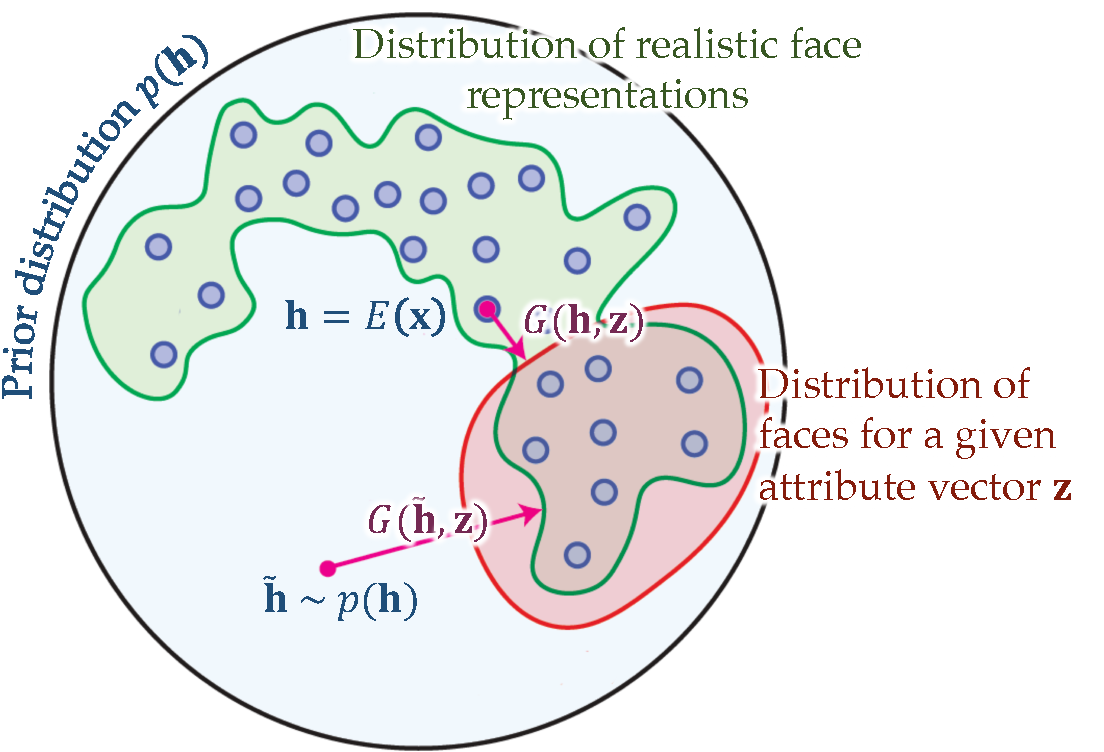
\includegraphics[width=0.72\textwidth]{images/dualdis_engel}
    \titlecaption{Behavior of Latent Constraint \acs{VAE} by \citet{engel2018latent}}{They learn a model $G(\vz,\vz)$ that is capable of transforming an existing representation $\vh$ (encoded from an image or sampled randomly) into a realistic image that is valid regarding the provided attributes $\vz$. {\small Credits: Illustration based on \citet{engel2018latent}}}
    \label{dualdis:fig:engel}
\end{figure}

To overcome this and control semantic factors, the most simple way is to use conditional generation, which consists in generating from a noise $\vht$ and a label vector $\vz$, as proposed by \citet{perarnau2016invertible,wang2018high,Bodla2018,he2019attgan} and many others. While effective, it seems clear that all the complex information related to a semantic factor (\eg the glasses on a picture of a face) cannot be fully represented by a binary representation. Thus, that part of this information must leak into $\vht$. This is why trying to find richer representations of the semantic factors is an important direction.

An interesting idea in this direction to model more complex representations of semantic factors is proposed by \citet{engel2018latent} and is illustrated in \autoref{dualdis:fig:engel}. They start with a regular trained \ac{VAE} model that encoded the dataset without supervision. Making the hypothesis that the information about semantic factors has been somewhat organized in the latent space $\vh$ of the \ac{AE}, they add a model $G(\vh, \vz)$ which role will be to represent how the semantic information is organized in $\vh$. More precisely, $G$ is trained to transform any representation $\vh$ into a representation $\vh'$ that is ``valid'' with regard to the label vector $\vz$: $\vh'=G(\vh,\vz)$. For example, if $\vh$ represents someone without glasses, the glasses can be added using a vector $\vz$ with glasses set to true. $G$ should produce a new vector $\vh'$ keeping the same identity but adding glasses. The role of $G$ is therefore to model how each semantic factor $\vz_i$ has been represented and organized in the latent space $\vh$ by the original \ac{VAE}. Unlike a conditional model, the information about $\vz$ is represented directly in $\vh$ and $G$ allows finding regions of $\vh$ corresponding to factors $\vz$.

\subsection{Unsupervised disentangling}\label{dualdis:sec:RW_unsup}

The disentangling literature proposes to go further on this idea of structuring the information in the latent space. ``Disentangling'' can have more or less constraining definitions depending on the articles, but overall it consists in explicitly separating and representing independent factors of variation.

A first approach is unsupervised disentangling, where no labels about the factors of variation are provided. Those approaches are usually based on \acp{VAE} and try to produce a model in which latent units are all independent of each other. A simple solution is for example $\beta$-\ac{VAE} by \citet{higgins2017beta}, which adds a weighting parameters $\beta$ on the prior constraint, increasing how independent the latent neurons are. \citet{chen2018isolating,kim2018disentangling} both study this phenomenon more thoroughly by decomposing the prior term into multiple terms and increasing only the importance of the \textit{total correlation} term in their models FactorVAE and TC-VAE. Finally, \citet{dupont2018learning} proposes a variant which allows discrete intermediate representation in $\vh$.

Those models are based on the assumption that each latent unit encodes one variation factor and that all the units are independent of each other. To actually quantify this phenomenon, they all propose their own metrics to, \textit{in fine}, measure how well labeled variation factors (used only for evaluation) are represented, each in a single neuron of $\vh$. This definition (and metric) of disentangling is of course widely discussed \citep{higgins2018towards}. For example, it is not clear why a semantic factor should only be encoded by a single neuron, and whether it is realistic to consider only independent neurons and factors.

Other models differ from this ``disentangling by regularization'' approaches based on \ac{VAE}. For example, \citet{Kulkarni2015,Hu2018} work on latent chunks, \ie groups of neurons of $\vh$ that should each encode a semantic piece of information. In particular, \citet{Hu2018} propose to mix latent chunks of different images and adversarially enforcing similarity and difference of images generated from the mixes to obtain disentangling and independent chunks.

However, unsupervised disentangling has two important issues: first, without any supervision, it is not easy to enforce that a model actually learns complex semantic factors (\textit{e.g.} facial expression, pose, hairstyle, \textit{etc.}) and not for example a decomposition of the factor into an ensemble of simpler and less semantic ones. This is especially true when enforcing that each neuron encodes a different factor. Second, because we don't have labels, it is impossible to interpret the latent representations, the only solution being to ask a human to look at the effect of each neuron and visually interpret it, which is risky regarding the generalization on the full dataset of the interpretation made on a few samples. Besides, if a human needs to label the representations, it seems more reasonable to use this time to label the factors in the dataset and use them in the training.

\subsection{Supervised disentangling}

Numerous approaches also propose \textit{supervised disentangling}, using labels in addition to images to disentangle factors of variation. In this literature, the definition of disentangling is even broader than for \textit{unsupervised disentangling}, focusing on separating different pieces of information.

A first approach for this is based on conditional generative models, where the decoder takes $(\vh, \vz)$ as input, where $\vz$ are the labeled factors and $\vh$ represents the rest of the information. In this regard, we can cite \citet{perarnau2016invertible,Tran2017,Liu2018}. A good example is Fader Network \citep{Lample2017}, which uses an \acs{AE}-based model: the encoder producing $\vh$ is supposed to represent everything (mostly the identity and the background) except the visual attributes (makeup, hairstyle, glasses, \etc); the decoder takes $\vh$ and the attributes as a binary vector $\vz$ as input to reconstruct. The disentangling between attributes and non-attributes is achieved by forcing the encoder to remove $\vz$-related information in $\vh$ using adversarial training.

Numerous approaches are also based on an approach similar to the intuition of HybridNet, separating the information in two latent spaces. This is the case of \citet{Mathieu2016,peng2017reconstruction,Klys2018,Hadad2018,Jaiswal2018,Liu2018a}. The general idea of those models is to find a way to separate two information domains (\eg information related to a person's identity $\vy$ and information related to visual attributes $\vz$ of a face) in two latent spaces. Mostly, it consists in using classification and adversarial training to represent $\vy$-related information in one subspace and remove $\vy$-related information in the other subspace. These methods can be reproduced using parts of our DualDis framework and will be discussed in depth in \autoref{dualdis:sec:discussion}.


\section{DualDis approach} \label{dualdis:sec:model}

\begin{sidewaysfigure}[p]
    \centering
    \hspace*{-2cm}
    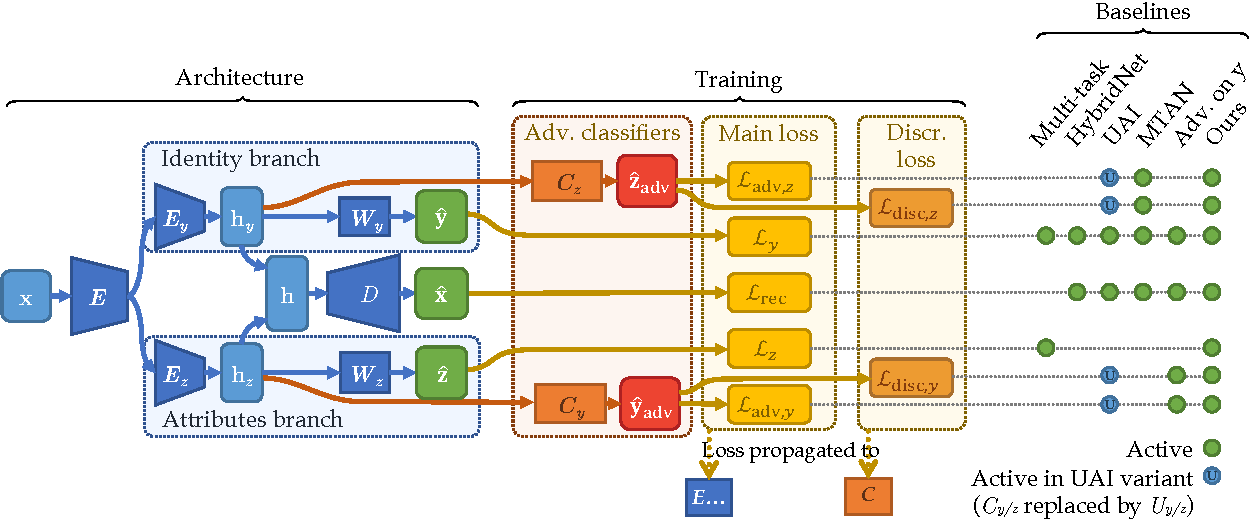
\includegraphics[width=\linewidth]{images/dualdis_archi.pdf}
    \hspace*{-2cm}
    \titlecaption{Architecture and learning of the DualDis framework}{We use a two-branch encoder-decoder architecture with classifiers (left). For the training, in addition to classical reconstruction and classification losses, we use adversarial classifiers and loss terms to force the two latent spaces to encode complementary ``orthogonal'' information (middle).
    We also indicate (right) how subsets of components of DualDis can be used to reproduce existing baselines described in \autoref{dualdis:sec:discussion}, in particular Multi-task models \citep{kokkinos2017}, HybridNet, UAI \citep{Jaiswal2018}, MTAN \citep{Liu2018}, models with an adversarial loss on $\vy$ only \citep{Hadad2018,Liu2018a,Klys2018}.}
    \label{dualdis:fig:archi}
\end{sidewaysfigure}

In this chapter, we propose to build upon the intuitions and interpretations of HybridNet to address supervised disentangling. Our objective is to separate two \textit{information domains} that are complementary: the first represents the class or person's identity $\vy$, \ie a category that contains a lot of intra-class variability, and the second domain represents semantic attributes $\vz$ (\eg hairstyle, makeup, pose, lighting, \etc) related to this variability.

To this end, we propose an approach called DualDis presented in \autoref{dualdis:fig:archi}. On the left, we show the architectural part of our contribution, using a two-branch model and disentangling to separate the two information domains. Those domains have classification labels $\vy$ and $\vz$ that we want to predict ($\vyh$, $\vzh$), along with a reconstruction $\vxh$ of the input $\vx$. In the center of the figure, we describe the second part of our approach which is the training process designed to successfully disentangle the two domains, using adversarial classifiers and multiple loss terms. On the right, to put our model in perspective, we indicate how some related works can be reproduced using the same kind of architectures with variations in the losses used as described in \autoref{dualdis:sec:discussion}.

In this section, we will detail how DualDis is designed to separate the information domains and linearize semantic factors. For information separation, each latent space is connected to an adversarial classifier of the opposite information domain which learns to find the information that belongs to the wrong domain. The encoder will then learn to remove this information from the latent space, making classification impossible and thus filtering only the relevant information. DualDis is also designed to linearize the labeled factors. We use linear classifiers that both guide the linearization process and provide us with the linear directions that are associated with known labeled semantic factors. This allows us to semantically navigate the latent spaces since moving in one of those linear directions will increase the presence of the associated factor.


\subsection{Dual branch Auto-Encoder}\label{dualdis:sec:model_ae}

We propose an encoder-decoder architecture with a latent space split into two parts, $\vhy$ and $\vhz$. Each representation is produced by a deep encoder $E_y$ or $E_z$ so that the features are explicitly separated. These representations are concatenated into $\vh$ and fed to a decoder $D$, producing a reconstruction $\vxh$. Having a decoder enables image generation and also ensures that the model extracts robust features \citep{le2018supervised} as we have seen in the previous chapters.

While it would be possible to encode all the information in a single latent space, having two branches encourages the model to encode two complementary kinds of information \citep{Mathieu2016,Hadad2018,Liu2018}. Taking the example of a face dataset, we want the identity branch ($E_y \circ E$) to capture information related to the identity $\vy$ with invariance toward other factors of variation (hairstyle, makeup, pose, \textit{etc.}); and we want the attribute branch ($E_z \circ E$) to model this ignored information, since this branch needs to capture factors of variation linked to visual attributes $\vz$. Having two separate deep encoders $E_y$ and $E_z$ is key to an effective disentangling, and they should be designed deep enough to produce ``orthogonal'' latent representations that encode very different information. Since the low-level features represented by the first convolutional layers are likely common to both domains, we use a single common encoder $E$ before specializing the information in our two branches.

This auto-encoding backbone is trained using a simple \ac{MSE}, $\calL_\textrm{rec} = ||\vx - \vxh||_2^2$. Using a different loss to train the decoder could be possible, like using a GAN discriminator \citep{Goodfellow2014} or a perceptual loss \citep{dosovitskiy2016generating} which are both known to produce sharper images. However, we considered that it was out of the scope of this work since we are not interested in producing high-quality generations but focus on the disentangling ability of the model.


\subsection{Modeling factors of variation}\label{dualdis:sec:model_factors}

We want our architecture to produce robust representations of each information domain as well as provide classification predictions. To that end, we have seen in the previous chapter that having a two-branch encoder can improve classification performance by encouraging representations $\vhy$ and $\vhz$ to be invariant toward intra-class variations. To the encoders, we add linear classifiers $\vW_y$ and $\vW_z$, one for each branch, that predicts respectively $\vyh$ and $\vzh$. These classifiers guide the auto-encoding backbone to organize the information extracted for reconstruction in the right branch between our two latent spaces $\vhy$ and $\vhz$ so that it allows predicting the class/identity and the attributes. To train those classifiers, we use regular classification losses. We have:
\begin{align}
    \vyh &= \softmax(\vW_y \vhy) \,, & \vzh &= \sigmoid(\vW_z \vhz) \,; \\
    \calL_{y} &= \textrm{CrossEntropy}(\vy, \vyh)         \,, &
    \calL_{z} &= \textrm{BinaryCrossEntropy}(\vz, \vzh)   \,.
\end{align}

\paragraph{Linearization of the factors for manipulation.} In addition, the design of those classifiers is chosen in order to encourage the linearization of the representations of labeled factors of variation. By choosing linear classifier, the presence of the $i^\text{th}$ attribute $\vz_i$ in an input image is estimated by a linear predictor:
\begin{equation}
    \vzh_i = \sigmoid(\vw_{z_i} \cdot \vhz)\text{ with }\vw_{z_i}\text{ the }i^\text{th}\text{ row of the matrix }\vW_z\, .
\end{equation}
This means that we can manipulate the latent space to artificially increase or decrease the presence of this attribute by moving $\vhz$ in the direction of this vector:
\begin{equation}
    \vhz' = \vhz \pm \varepsilon \vw_{z_i}^\top\,.
\end{equation}

\subsection{Disentangling information domains and factors of variation}\label{dualdis:sec:model_dis}

We also want our architecture to explicitly disentangle the two domains. To this end, we add classifiers $C_y(\vhz)$ and $C_z(\vhy)$ that predict the target of the opposite domain ($\vy$ from $\vhz$ and vice versa). We call those classifiers ``adversarial'' since their role is to find information that should not be present, \textit{e.g.} information about attributes encoded in the identity branch. By training a classifier to find this information, we are then able to make the encoder remove it. Those classifiers are designed as non-linear multi-layer classifiers to find the information even if it is not linearly separable in the latent space.

\subsubsection{Global loss and adversarial training}

To train our model, we rely on adversarial training, with parts of the model that have different training losses but are connected. Concretely, it means that the parameters of the model are not all updated using the same losses, as is represented in \autoref{dualdis:fig:archi}.

We define $\theta_\mathrm{main}$ as the weights of the \textit{main} model, \ie the model that is eventually used at the end of the training, which includes the encoders, the decoder and the normal classifiers: $E,E_y,E_z,D,\vW_y,\vW_z$. We also define $\theta_\mathrm{disc}$ as the weights of the two adversarial classifiers $C_y$ and $C_z$ (similarly to \acp{GAN} denomination).

To train the model, we have two losses: \textit{main loss} $\calL_\mathrm{main}$ describes the expected behavior of the model and is propagated in the encoders, decoder and classifiers $\vW$. The \textit{discriminative loss} $\calL_\textrm{disc}$ is used to train the adversarial classifiers $C_y$ and $C_z$ only; helping the main loss by searching for information that should be removed.
\begin{align}
    \calL_\mathrm{main} &= \lambda_r \calL_\textrm{rec} + \lambda_y \calL_{y} + \lambda_z \calL_{z} + \lambda_{a,y} \calL_{\textrm{adv},y} + \lambda_{a,z} \calL_{\textrm{adv},z} + \lambda_{o} \calL_\textrm{orth}\,,\\
    \calL_\mathrm{disc} &= \lambda_{d,y} \calL_{\textrm{disc},y} + \lambda_{d,z} \calL_{\textrm{disc},z}\,.
\end{align}
Each loss term in these global losses can be weighted using various $\lambda$ to control their importance.

To optimize our model, we apply a gradient descent using backpropagation, which for \acs{SGD} writes:
\begin{align}
    \theta_\mathrm{main} &\leftarrow \theta_\mathrm{main} - \eta \nabla_{\theta_\mathrm{main}} \calL_\mathrm{main}\,, \\
    \theta_\mathrm{disc} &\leftarrow \theta_\mathrm{disc} - \eta \nabla_{\theta_\mathrm{disc}} \calL_\mathrm{disc}\,.
\end{align}
Interestingly, we can see that to compute the gradients, we apply backpropagation to layers that are not necessarily updated by the optimizer, which is unusual in \ac{DL} outside of adversarial learning.

\subsubsection{Disentangling information domains}

To effectively remove information where it should not be encoded, we thus start by defining discriminative loss terms $\calL_{\textrm{disc},y}$ and $\calL_{\textrm{disc},z}$, applied to $C_y$ and $C_z$, to make the adversarial classifiers achieve the correct classification of their target. These will make the adversarial classifiers model the information we want to remove.

We then define the adversarial terms $\calL_{\textrm{adv},y}$ and $\calL_{\textrm{adv},z}$ in the main loss to make the encoders produce features that prevent the classifiers $C$ to achieve their goal and ideally have the accuracy of a random classifier. This means that the encoders will need to remove the information that is used by the classifiers $C$, which is unwanted. This goal can be expressed in different possible ways:
\begin{itemize}
    \item $\max \Ent[\vyhadv]$ \\
    By maximizing the entropy of the adversarial prediction, which is optimal when the classifier assigns the same probability to all the classes.
    \item $\min \textrm{CrossEntropy}(p_\mathrm{prior}(\vyhadv), \vyhadv)$\\
    By minimizing the cross-entropy with a prior distribution $p_\mathrm{prior}(\vyhadv)$ for which we have different options: a uniform distribution among the classes (which has the same optimum as $\max H[\vyhadv]$ but different gradients); a distribution that matches the prior distribution of the classes in the dataset if it is unbalanced; \etc.
    \item $\max \textrm{CrossEntropy}(\vy, \vyhadv)$\\
    By simply encouraging the prediction of the ``inverse'' of the ground truth, \ie maximizing the cross-entropy with the ground truth. While being less mathematically correct since it means the optimum would be to predict a probability score of the ground truth class lower than the other classes, we found this solution to be  the most effective, probably because it has better gradients and since in practice it is actually never able to reach the point where the probability of the real class is lower than the others.
\end{itemize}

Thus, we choose to use the following loss terms:
\begin{align}
    \calL_{\textrm{disc},y} &= \textrm{CrossEntropy}(\vy, \vyhadv) \,,    \\
    \calL_{\textrm{adv},y} &= -\textrm{CrossEntropy}(\vy, \vyhadv) \,;   \\[0.5em]
    \calL_{\textrm{disc},z} &= \textrm{BinaryCrossEntropy}(\vz, \vzhadv) \,,\\
    \calL_{\textrm{adv},z} &= \textrm{BinaryCrossEntropy}(1-\vz, \vzhadv) \,.
\end{align}

\subsubsection{Intra-branch disentangling}

Using adversarial classifiers, we disentangled class and attribute features. We now propose to disentangle the different labeled factors of variation by making the rows of the matrix $\vW_z$ orthogonal, meaning each factor detector is independent of the others. We do so by minimizing the dot products of the pairs of normalized row vectors $\vw_{z_i}'$ of $\vW_z$:
\begin{equation}
    \calL_\mathrm{orth} = \sum_i \sum_j \vw_{z_i}' \vw_{z_j}'^{\top} \quad\text{ with }\quad \vw_{z_i}' = \frac{\vw_{z_i}}{||\vw_{z_i}||_2} \,.
\end{equation}

% Define numbering of the baselines for use in text and table
\newcommand{\MTHNref}{(A\,\&\,B)\xspace}
\newcommand{\MTref}{(A)\xspace}
\newcommand{\MTANref}{(C)\xspace}
\newcommand{\HNref}{(B)\xspace}
\newcommand{\HNpref}{(B')\xspace}
\newcommand{\HNrefs}{(B\,\&\,B')\xspace}
\newcommand{\UAIref}{(D)\xspace}
\newcommand{\UAIrefs}{(D\,\&\,D')\xspace}
\newcommand{\UAIpref}{(D')\xspace}
\newcommand{\Yref}{(E)\xspace}

\section{Discussion}
\label{dualdis:sec:discussion}

Let us now discuss our DualDis approach in regard to related works and existing state-of-the-art models of supervised disentangling. 
Interestingly, as shown in \autoref{dualdis:fig:archi} (right), several existing state-of-the-art disentangling models can be reproduced and evaluated using the same architecture and loss components. By disabling parts of our architecture and/or with small additions and variations, we can thus produce a complete and fair comparison to them. We assign letters (A) to (E) to those models as we will refer to them in the experiments.

\paragraph{Class-only adversarial disentangling \Yref.}

First, by starting with Dual\-Dis and removing losses related to the attribute labels $\vz$, we obtain \textit{model~\Yref} that learns to predict the class $\vy$ in one branch and dispel the information related to $\vy$ in the other. This is notably the case for the recent models by \citet{Hadad2018,Liu2018a,Klys2018}.

The advantage compared to DualDis is that fewer annotations are required. However, this means that the disentangling is asymmetrical: while identity-related information is constrained, the attribute-related information remains unconstrai\-ned and can thus be encoded freely in $\vhy$ and $\vhz$ and remain entangled. It is therefore very difficult to ensure proper separation of the two information domains with this asymmetry. Besides, without labels $\vz$, we lack a way to semantically navigate in the latent space $\vhz$. This is why we choose strong supervision with labels for both $\vy$ and $\vz$.

\paragraph{Symmetric latent adversarial disentangling \UAIref.}

To solve this asymmetry, UAI \citep{Jaiswal2018} proposes a new adversarial training used as \textit{model~\UAIref}, still without attribute labels. In their model, adversarial predictors $U_y$ and $U_z$ replace $C_y$ and $C_z$. Those predictors learn to predict $\hat{\vh}_y$ from $\vhz$ and vice versa, \textit{i.e.} the opposite latent space. The encoders try to fool those predictors and make them fail at their prediction. Because no labels are needed for this task, this can be trained in an unsupervised manner. Probably due to the complexity of the predictor's task, all the modules (encoders, predictors, decoder) in \citet{Jaiswal2018} are linear.

This idea has the advantage of being symmetrical even without attribute labels, but it only ``orthogonalizes'' $\vhy$ and $\vhz$, making them independent of each other, but without guarantee of semantic disentangling. In particular, nothing ensures attribute information is removed from $\vhy$, since for it to happen, the model would need to encoded attribute information in $\vhz$ without labels. In addition, identity information can even remain in $\vhz$ if absent from $\vhy$. This is why we choose an explicit disentangling of labeled information.

\paragraph{Attribute-conditional decoder \MTANref.} Some models like Fader Networks \citep{Lample2017}, IcGAN \citep{perarnau2016invertible}, or MTAN \citep{Liu2018} \textit{(model~\MTANref)} propose to use a \textit{conditional generator} approach, which a single latent space $\vhy$ to encode the identity and a decoder fed with a binary vector $\vz$: $D(\vhy, \vz)$. MTAN in particular applies a classification loss on $\vy$ and an adversarial loss on $\vz$ to remove the attribute information from $\vhy$.

Simplifying the disentangling since $\vz$ is by definition purely attribute information and we only need to remove attribute information from $\vhy$, this approach has other drawbacks. Notably, it makes the strong assumption that all the attribute information of a specific image is encoded in the binary vector $\vz$, which is unlikely for complex semantic attributes, like a pair of glasses, a hat, facial expression, age, \textit{etc.} This means that attributes information will necessarily leak in $\vhy$, and that our control on the attribute is very simple since we cant only control a binary value. This is why we prefer to use two latent spaces to let the model encode complex information in both information domains.

\paragraph{Multi-Task Learning \MTHNref.} Finally, while not explicitly designed for it, two-branch multi-task models could also lead to disentangling thanks to the specialization induced by classification, even without adversarial training. In particular, we consider two possible setups. First, a model that learns to classify $\vyh$ and $\vzh$ like UberNet \citep{kokkinos2017} \textit{(model \MTref)}. And second, a simple variation of HybridNet \textit{(model \HNref)}, that both learn to classify $\vyh$ while encoding additional information in $\vhz$, and simultaneously learn to reconstruct to extract additional information not present explicitly in the labels.
Compared to those methods, we choose to integrate an explicit disentangling process to effectively separate the information domains.

\FloatBarrier

\section{DualDis evaluation}
\label{dualdis:sec:exp}

We now propose to validate the effectiveness of our DualDis approach to efficiently disentangle two information domains. In this section, we describe the datasets used for this as well as the evaluation metrics that we use to quantitatively measure the disentangling and linearization performance of the models. We evaluate DualDis and compare it to state-of-the-art techniques previously described.

In \autoref{dualdis:sec:ssl}, we present and evaluate own DualDis can be adapted to a semi-supervised context. In \autoref{dualdis:sec:editing}, we perform a qualitative evaluation of the possibility to perform image editing and use this capability to generate new images for \acf{DA}.

\subsection{Datasets and architecture}

\begin{table}[t]
    \centering
    \renewcommand{\arraystretch}{1.9}
    \begin{tabular}{@{}lcccccc@{}}
      \toprule \\[-2.9em] % removes the large stretch for the header
      Dataset & Image size & \# Train & \# Test & $|\mathcal Y|$ & $|\mathcal Z|$ & Samples \\[-0.25em]
      \midrule
      CelebA   & 256$\times$256 & 48,000 & 12,000 & 2,000 & 40 & 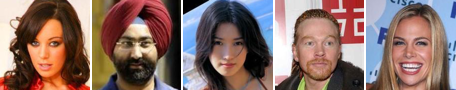
\includegraphics[align=c,width=5.2cm]{images/dataset_celeba} \\
      Yale-B   & 64$\times$64   &  1,200 &  1,200 & 38 & 14 & 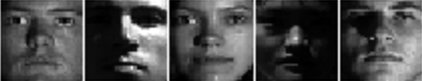
\includegraphics[align=c,width=5.2cm]{images/dataset_yale} \\
      NORB     & 64$\times$64   & 24,000 & 24,000 & 5 & 8 & 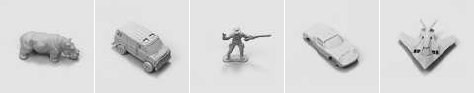
\includegraphics[align=c,width=5.2cm]{images/dataset_norb} \\
      \bottomrule
    \end{tabular}
    \titlecaption{Overview of the datasets used}{We report the size of the images, the number of samples used for training and testing, the number of classes $|\mathcal Y|$ in $\vy$ and the number of attributes $|\mathcal Z|$ in $\vz$.}
    \label{dualdis:tab:datasets}
  \end{table}

For the experiments, we use three datasets (\cf \autoref{dualdis:tab:datasets}) preprocessed to fit our training protocol:
\begin{itemize}
    \item \textbf{CelebA} \citep{celeba} is a face dataset of celebrities, for which we use 60k images with 2000 identities $\vy$ and 40 attributes $\vz$ (hairstyle, makeup, expression, \textit{etc.}).
    \item \textbf{Yale-B} \citep{yale} is also a face dataset of 2.4k images with 38 identities $\vy$ and 14 attributes $\vz$ (light source position). More precisely, each of the 38 persons has been photographed once with 64 possible lighting combinations which we grouped into 14 categories of lightning.
    \item \textbf{NORB} \citep{norb} is a dataset of 3D object renderings. 50 objects are rendered with different camera position and lighting type (960 combinations per object), making a dataset of 48k images with 5 categories $\vy$ (10 objects per category) and 8 attributes $\vy$ (camera position and lighting, created by us by grouping similar angles and lightings).
\end{itemize}

For CelebA and Yale-B, we create a test set by using respectively 20\% and 50\% of the images of each class, regardless of the attributes. For NORB, the test set is provided and consists of 25 of the 50 3D objects which represent 50\% of the images. The validation set represents 20\% of the training set, defined with the same process, and is used for the few hyper-parameters tests we do.

For the architecture, we use simple \acp{ConvNet} inspired by exiting models used in the literature. Encoders and decoders are composed of convolutional layers interlaced with \ac{BN} and \acs{ReLU} activations. Spatial information is aggregated using strided convolutions in the encoders, and is recreated in the decoded with nearest neighbor upsampling. The depth of the encoders and decoders depends on the dataset: the encoders range from 6 to 8 layers, decoders between 7 and 13 layers and latent spaces $\vhy$ and $\vhz$ are 80 to 196 units.

Finally, we can note that our model is not really sensitive to the hyperparameters $\lambda$, which were set with logical values (depending on the importance of the loss terms) and with validation tests. Also, the adversarial training does not present particular instabilities like can be encountered with \acp{GAN}, since we did not had issues during our experiments. The exact details about the data preprocessing, the architectures used and the training information is provided in \autoref{chapter:dualdisA}. 


\begin{table}[p] % sidewaystable
    \centering

    \begin{adjustbox}{scale=0.97}
    \setlength{\tabcolsep}{6pt}
    \hspace*{-2cm}
    \begin{tabular}{@{}ll@{\hspace{4pt}}ll@{\hspace{15pt}}c@{\hspace{20pt}}cc@{\hspace{13pt}}cc@{}}
        \toprule
    &&                             & Labels             & Aggr.  & \multicolumn{2}{c}{Accuracy} &  \multicolumn{2}{c}{Disentangling} \\
   && Model                        & used               & metric 
                                & ${\scriptstyle \vh_{\scriptstyle y} \rightarrow} \vy$     
                                & ${\scriptstyle \vh_{\scriptstyle z} \rightarrow} \vz$    
                                & ${\scriptstyle \vh_{\scriptstyle z} \rightarrow} \vy_\textrm{adv}$
                                & $\!\!{\scriptstyle \vh_{\scriptstyle y} \rightarrow} \vz_\textrm{adv}$ \\
\midrule

\parbox[t]{3mm}{\multirow{8}{*}{\rotatebox[origin=c]{90}{\textbf{CelebA}}}}
&          & \textit{Dataset prior}             &                             &          &            &            & \itshape 99.5\% & \itshape 19.5\% \\
& \MTref   & Multi-task classif.                & \okI, \okA                  &     61.1 & \bf 77.6\% & \bf 91.8\% &     65.5\% & \,\  9.5\% \\ % 77.6, 34.5, 91.8, 90.5
& \HNref   & HybridNet-like                     & \okI                        &     65.1 &     73.0\% &     82.4\% &     95.5\% & \,\  9.4\% \\ % 73.0,  4.5, 82.4, 90.6
& \HNpref  & HybridNet-like + attr              & \okI, \okA                  &     65.2 &     72.7\% &     90.1\% &     88.5\% & \,\  9.5\% \\ % 72.7, 11.5, 90.1, 90.5
& \MTANref & MTAN                               & \okI, \okA, \okAt           &      --  &     68.9\% &        --  &        --  &     13.8\% \\ % 68.9,  NaN,  NaN, 86.2
& \UAIref  & UAI  adv. loss                     & \okI                        &     63.7 &     67.9\% &     80.3\% & \bf 97.3\% & \,\  9.3\% \\ % 67.9,  2.7, 80.3, 90.7
& \UAIpref & UAI  adv. loss + attr              & \okI, \okA                  &     65.0 &     68.0\% &     89.4\% &     92.9\% & \,\  9.5\% \\ % 68.0,  7.1, 89.4, 90.5
& \Yref    & Adv. on $\vy$ only                 & \okI                        &     64.7 &     69.2\% &     83.6\% &     96.4\% & \,\  9.6\% \\ % 69.2,  3.6, 83.6, 90.4
&          & \textbf{DualDis}                   & \okI, \okA                  & \bf 68.0 &     71.1\% &     88.6\% & \bf 97.3\% & \bf 14.9\% \\ % 71.1,  2.7, 88.6, 85.1

\midrule
\parbox[t]{3mm}{\multirow{8}{*}{\rotatebox[origin=c]{90}{\textbf{Yale-B}}}}
&          & \textit{Dataset prior}             &                             &          &            &            & \itshape 97.4\% & \itshape 92.9\% \\
& \MTref   & Multi-task classif.                & \okI, \okA                  &     81.5 &     98.5\% &     97.2\% &     85.3\% &     45.1\% \\ % 98.5, 14.7, 97.2, 54.9
& \HNref   & HybridNet-like                     & \okI                        &     65.3 &     97.6\% &     93.7\% &     23.3\% &     46.5\% \\ % 97.6, 76.7, 93.7, 53.5
& \HNpref  & HybridNet-like + attr              & \okI, \okA                  &     80.5 & \bf 99.0\% &     96.9\% &     80.0\% &     46.1\% \\ % 99.0, 20.0, 96.9, 53.9
& \MTANref & MTAN                               & \okI, \okA, \okAt           &      --  &     98.4\% &        --  &        --  &     70.3\% \\ % 98.4,  NaN,  NaN, 29.7
& \UAIref  & UAI  adv. loss                     & \okI                        &     60.0 &     98.6\% &     65.5\% &     28.1\% &     48.0\% \\ % 98.6, 71.9, 65.5, 52.0
& \UAIpref & UAI  adv. loss + attr              & \okI, \okA                  &     65.1 &     96.1\% &     95.8\% &     44.4\% &     24.1\% \\ % 96.1, 55.6, 95.8, 75.9
& \Yref    & Adv. on $\vy$ only                 & \okI                        &     79.8 &     98.3\% &     84.1\% &     92.5\% &     44.4\% \\ % 98.3,  7.5, 84.1, 55.6
&          & \textbf{DualDis}                   & \okI, \okA                  & \bf 92.0 &     98.6\% & \bf 97.3\% & \bf 98.8\% & \bf 73.4\% \\ % 98.6,  1.2, 97.3, 26.6

\midrule
\parbox[t]{3mm}{\multirow{8}{*}{\rotatebox[origin=c]{90}{\textbf{NORB}}}}
&          & \textit{Dataset prior}             &                             &          &            &            & \itshape 80.0\% & \itshape 31.3\% \\
& \MTref   & Multi-task classif.                & \okI, \okA                  &     53.7 &     93.0\% &     84.2\% &     13.5\% &     24.0\% \\ % 93.0, 86.5, 84.2, 76.0
& \HNref   & HybridNet-like                     & \okI                        &     51.1 &     93.3\% &     76.8\% &     12.2\% &     22.1\% \\ % 93.3, 87.8, 76.8, 77.9
& \HNpref  & HybridNet-like + attr              & \okI, \okA                  &     52.5 &     92.9\% &     84.1\% &     10.7\% &     22.2\% \\ % 92.9, 89.3, 84.1, 77.8
& \MTANref & MTAN                               & \okI, \okA, \okAt           &      --  &     92.2\% &        --  &        --  & \bf 30.5\% \\ % 92.2,  NaN,  NaN, 69.5
& \UAIref  & UAI  adv. loss                     & \okI                        &     51.8 &     92.8\% &     76.0\% &     13.7\% &     24.7\% \\ % 92.8, 86.3, 76.0, 75.3
& \UAIpref & UAI  adv. loss + attr              & \okI, \okA                  &     52.5 &     93.2\% &     82.8\% & \,\  8.0\% &     26.0\% \\ % 93.2, 92.0, 82.8, 74.0
& \Yref    & Adv. on $\vy$ only                 & \okI                        &     67.3 &     92.2\% &     76.9\% &     78.9\% &     21.1\% \\ % 92.2, 21.1, 76.9, 78.9
&          & \textbf{DualDis}                   & \okI, \okA                  & \bf 72.3 & \bf 93.5\% & \bf 84.5\% & \bf 80.7\% & \bf 30.5\% \\ % 93.5, 19.3, 84.5, 69.5

        \bottomrule
    \end{tabular}
    \hspace*{-2cm}
\end{adjustbox}
\titlecaption{Comparison to state-of-the-art models}{We indicate the labels necessary in train ($\vy, \vz$) and to use the model ($\vz_\mathrm{eval}$). We measure the \textit{accuracy} of the classifiers $\vW_y(\vhy)$ and $\vW_z(\vhz)$ to predict the classes and attributes; and the \textit{disentangling quality} as the error rate (100 - accuracy) of the classifiers $C_y(\vhz)$ and $C_z(\vhy)$ indicating if the information was correctly removed.
    Our \textit{aggregated metric} is an average of the four scores to indicate the overall performance. For all the scores, \textit{higher is better}.
    The \textit{dataset prior} scores show the highest disentangling score that we can obtain considering the prior on the distribution of the dataset.
    }
    \label{dualdis:tab:sota}
\end{table}


\subsection{Quantitative evaluation}
\label{dualdis:sec:exp_dis}

We now study the ability of DualDis to successfully disentangle and linearize the factors of variation of the two information domains (class/identity and attributes) in the latent spaces.
To do so, we compare our model to baselines described in \autoref{dualdis:sec:discussion} that are reproduced similarly to an ablation study by deactivating components of our model or by making small changes, \textit{cf.} \autoref{dualdis:fig:archi}. We can therefore compare our model to fair reimplementations of the state of the art. We also evaluate variants of the baselines where labels are available for both information domains, like for DualDis. All models we train have the same architecture (in $E$, $E_y$, \textit{etc.}) and the same hyperparameters' values whenever those are common between models. Only UAI \citep{Jaiswal2018} has a slightly different architecture since it requires shallow encoders $E_y$ and $E_z$.\footnote{When using this architecture with shallow encoders with the other methods, we obtain the same trends as the ones we report, only with a small degradation to all the models.}

\paragraph{Evaluation metrics.} First, to evaluate the quality of the representations, we measure the \textit{accuracy} of the linear classifiers $\vW_y$ and $\vW_z$, which indicates both if the information regarding the labels is correctly extracted and if this information has been linearized to allow its manipulation. Second, to evaluate the disentangling of the information domains, we measure the \textit{error rate} (100 - accuracy) of the adversarial classifiers $C_y$ and $C_z$, which measures how much of the ``undesired'' information has been removed through disentangling.\footnote{For models that do not include classifiers $C$, we add and train them to obtain disentangling metrics, without impacting the behavior of the rest of the model, \textit{cf.} details in the appendix.} Of course, because a random classifier would not have an error rate of 100\%, this metric cannot reach this value. Finally, since both these metrics increase when they improve on our objective, we summarize the overall quality of a model with an \textit{aggregated metric} that averages those 4 values for a quicker interpretation of the results.

Note that the disentangling metric cannot go higher than a certain value that depends on the dataset. For example, if we want to remove information about a binary attribute $\vz$ present for 80\% of the examples, with a perfect disentangling, $C_z$ would predict this attribute randomly 80\% of the time, would have an accuracy of 80\% and thus a disentangling metric of 20\%. The best disentangling metric value is the error rate of a random classifier considering the distribution of the dataset. We indicate this value in the results for each dataset.



\paragraph{Comparison to the state of the art.}

Results are presented in \autoref{dualdis:tab:sota} with baselines described in \autoref{dualdis:sec:discussion} labeled (A) to (E).
%
DualDis provides the best performances on the three datasets with a gain of 3 to 10\,pts in the aggregated metric compared to the best baseline. Overall, we obtain strong disentangling results while having similar or better classification accuracies.

Looking at the baselines, first, the multi-task classifier \MTref \citep{kokkinos2017} provides good accuracies but completely fails at disentangling the information. This is probably because classification is made easier by not needing to compromise with reconstruction, that is not used in this model, also making generation impossible.
%
Adding reconstruction gives \HNrefs, which regularizes the model and slightly helps the disentangling metrics by grounding latent features to specific visual patterns in the reconstruction. In comparison, DualDis provides an explicit disentangling mechanism to greatly improve disentangling metrics.

MTAN~\MTANref \citep{Liu2018}, using a conditional generation approach, produces good results but uses a single latent space $\vhy$ and thus cannot be directly compared to DualDis. In particular, it is complicated to use in a real setup because it always requires labels $\vz$ as inputs of its decoder to be used, even in ``test'' (here meaning the use of the model after training). Besides, this constraint of encoding the attribute information in a binary vector causes lower quality reconstructions because this information cannot be represented in such a compact space.

Finally, we can see that the orthogonalization mechanism applied to latent representations proposed by UAI~\UAIrefs only produces weak disentangling results because of the strong limitations that we discussed. The most competitive disentangling results are provided by the asymmetrical disentangling of \Yref \citep{Liu2018a}, only applied to $\vy$. However, as we discussed, because of this asymmetry, it lacks the ability to correctly remove the attribute information in the identity space, with a disentangling metric on $\vz$ that is similar to the results of models that do not have any disentangling mechanism.

In comparison, we combine reconstruction for generation and features regularization; classification and linearization to improve the semantic quality of the features; and leverage symmetrical label-guided adversarial disentangling; and effectively separate the two domains in both latent spaces while having competitive classification results.


\FloatBarrier
\section{Semi-Supervised Learning}
\label{dualdis:sec:ssl}

\begin{table}[t]
    \centering
    \begin{tabular}{@{}r@{\hspace{12pt}}c@{\hspace{12pt}}cc@{\hspace{12pt}}cc@{}}
        \toprule
        Nb. attr.        & Aggr.                             &  \multicolumn{2}{c}{Accuracy} &  \multicolumn{2}{c}{Disentangling} \\
        labels        & metric                & ${\scriptstyle \vh_{\scriptstyle y} \rightarrow} \vy$     
                                    & ${\scriptstyle \vh_{\scriptstyle z} \rightarrow} \vz$    
                                    & ${\scriptstyle \vh_{\scriptstyle z} \rightarrow} \vy_\textrm{adv}$
                                    & ${\scriptstyle \vh_{\scriptstyle y} \rightarrow} \vz_\textrm{adv}$ \\
\toprule
            400   &     63.9 &     65.2\% &     81.2\% & \bf 97.7\% &     11.6\% \\ % 65.2,  2.3, 81.2, 88.4
            1000   &     65.5 &     68.4\% &     84.3\% &     97.4\% &     11.9\% \\ % 68.4,  2.6, 84.3, 88.1
            2000   &     66.8 &     71.0\% &     85.0\% & \bf 98.4\% &     12.7\% \\ % 71.0,  1.6, 85.0, 87.3
            4000   &     67.6 & \bf 72.6\% &     85.8\% & \bf 98.3\% &     13.8\% \\ % 72.6,  1.7, 85.8, 86.2
            48000  & \bf 68.0 &     71.1\% & \bf 88.6\% &     97.3\% & \bf 14.9\% \\ % 71.1,  2.7, 88.6, 85.1
        \bottomrule
    \end{tabular}
    \titlecaption{Results of disentangling on CelebA using \acf{SSL} on attribute labels}{``48k labels'' is the fully supervised baseline.}
\label{dualdis:tab:SSL}
\end{table}

The main drawback of DualDis is that it requires labels for both information domains, which can be expensive to annotate and is rarely the case in existing datasets. As we just saw in the previous section, using labels in both domains is critical for an effective disentangling. However, ideally, only a few labeled samples would be sufficient to guide the disentangling process of DualDis and provide semantic information on how the information is organized in the latent space.
%
Thus, to strongly minimize the need for annotations, we propose to explore the possibility of using \acf{SSL} in DualDis. As we saw in \autoref{chapter:hybridnet}, those methods can efficiently alleviate the need for labeled data with a relatively low cost. This would relax the constraint of having a fully labeled dataset for both domains, making the ``cost'' of applying this idea much lower.

A first and very simple ``\ac{SSL}'' strategy is to just ignore unlabeled samples whenever the label is necessary for a loss term. To go further and really apply state-of-the-art \ac{SSL} method to DualDis, the most relevant solutions are probably the techniques producing ``virtual'' targets like Temporal Ensembling \citep{Laine2016} or Mean Teacher \citep{tarvainen2017mean}, or label propagation-based methods \citep{iscen2019label}. Those methods would provide ground-truth-like vectors that could be used as classification targets whenever needed in the various loss terms.

We propose some preliminary experiments to investigate the possibility of obtaining disentangling and linearization of the domains using few attribute labels on CelebA. Using the same architecture as previously, we applied \ac{SSL} first by simply ignoring unlabeled samples when labels were needed, and second using the more advanced Mean Teacher strategy \citep{tarvainen2017mean}. We found, however, only a negligible difference in the results between the two. This is likely due to a sub-optimal tuning of the hyper-parameters of Mean Teacher which are very sensitive, as we noticed when working on HybridNet and confirmed by \citet{oliver2018realistic}.

Even with this simple strategy, we obtain interesting results that we report in \autoref{dualdis:tab:SSL}. Interestingly, we can see that even 1000 or 2000 labels --\,corresponding to 2 and 4\% of the train set size\,-- produce an aggregated score of 65.5 and 66.8, which is better than the baselines in \autoref{dualdis:tab:sota} and reasonably close to the model trained with full supervision. We also confirmed via a qualitative analysis of the model with 1000 labels that it can produce image edition and we obtained results visually similar to the ones of the fully supervised model in \autoref{dualdis:fig:celeba_change}. Applying \ac{SSL} to DualDis thus looks like a very promising idea.


\section{Image Editing and Data Augmentation}
\label{dualdis:sec:editing}

We now propose to evaluate two possible applications of this architecture provided by our encoder-decoder architecture and the ability to manipulate its latent representations: image editing and image generation for \acf{DA} on Yale-B.




\begin{figure}[tbp]
    \centering
    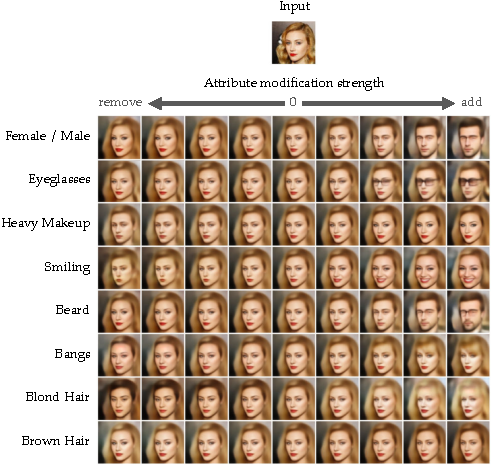
\includegraphics[width=\linewidth]{images/dualdis_celeba_linear.pdf}
    \titlecaption{Visualizations of progressive attribute editing on CelebA}{We do so by moving $\vhz$ with different strength $\varepsilon$ and in positive and negative directions along each vector $\vw_{z_i}$.}
    \label{dualdis:fig:celeba_linear}
\end{figure}
\begin{figure}[tbp]
    \centering
    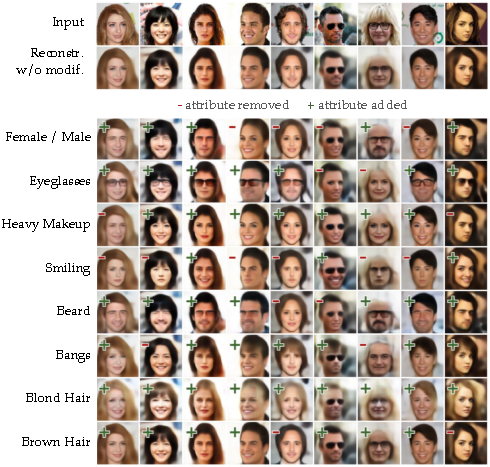
\includegraphics[width=\linewidth]{images/dualdis_celeba_change.pdf}
    \titlecaption{Visualizations of attribute inversion on CelebA}{For each image $k$ and each attribute $i$, we modify $\vhz\kk$ along the vector $\vw_{z_i}$ in the direction opposite to the ground truth label.}
    \label{dualdis:fig:celeba_change}
\end{figure}

\begin{figure}[p]
    \begin{subfigure}[b]{0.4\linewidth}
    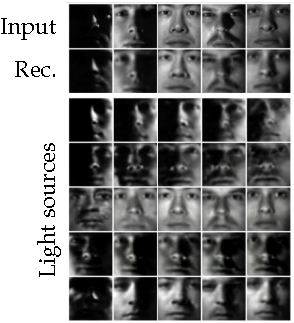
\includegraphics[width=0.9\linewidth]{images/dualdis_yale.pdf}
    \centering
    \titlecaption{Yale-B}{Our attributes correspond to the source of the light (from far right to far left when going down).}
    \label{dualdis:fig:yale}
    \end{subfigure}
    \hfill
    \begin{subfigure}[b]{0.57\linewidth}
    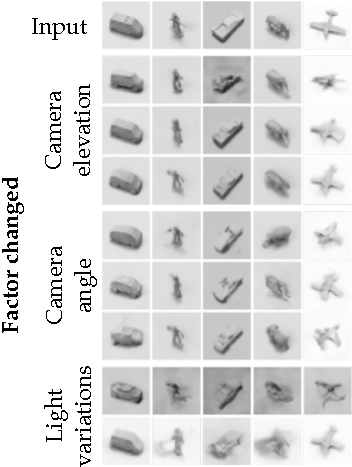
\includegraphics[width=0.76\linewidth]{images/dualdis_norb.pdf}
    \centering
    \titlecaption{NORB}{We change the camera elevation (from close to the ground to a view from above), the camera angle around the object and the intensity of light.}
    \label{dualdis:fig:norb}
    \end{subfigure}
    \titlecaption{Visualizations of image editing on Yale-B and NORB}{}
    \label{dualdis:fig:yale_norb}
\end{figure}
\begin{figure}[p]
    \centering
    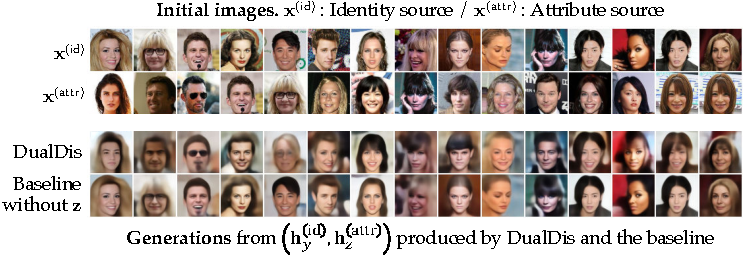
\includegraphics[width=\linewidth]{images/dualdis_celeba_mix.pdf}
    \titlecaption{Visualizations of the information separation through attribute and identity mix}{We show reconstructions using identity $\vhy$ from an image $\vx^{\mathrm{(id)}}$ and attributes $\vhz$ from an image $\vx^{\mathrm{(attr)}}$. We do this with our model and a baseline that do not use attribute labels for training \citep{Liu2018a}. We see that our model does use attributes from image $\vx^{\mathrm{(attr)}}$ while keeping the identity of image $\vx^{\mathrm{(id)}}$, whereas the baseline did not manage to remove attribute information from $\vhy$ and still uses attributes of image $\vx^{\mathrm{(id)}}$.}
    \label{dualdis:fig:celeba_mix}
\end{figure}

\subsection{Semantic image editing}

Using the disentangling and linearization abilities of DualDis, we perform semantic image manipulation by applying linear changes to $\vhz$ along attribute directions $\vw_{z_i}$. As explained in \autoref{dualdis:sec:model_factors}, we can add or remove an attribute like so:
\begin{equation}
    \vhz' = \vhz \pm \varepsilon \vw_{z_i}^\top\,.
\end{equation}

In \autoref{dualdis:fig:celeba_linear}, we show the visual effect of moving in positive and negative directions with different magnitudes for different attributes. This shows that we can finely control the importance of an attribute, increasing or decreasing its original presence on the image, until the attribute can eventually be considered removed or added. For example, we can add a small or big smile, choose among different shades of blonde hair, \etc.

For the next visualization in \autoref{dualdis:fig:celeba_change}, we fix a reasonable magnitude threshold for when an attribute is considered as changed (\ie added / removed). We then apply the method used above with this magnitude, in a direction chosen to flip the ground truth labels of different images for different attributes. Using this, we show that we can switch the gender, add and remove eyeglasses, hair bangs, \etc. A similar protocol was also used on Yale-B and NORB as shown in \autoref{dualdis:fig:yale_norb}. On those datasets though, because of the small size and variability in the datasets, even if the effect mostly remains, it is less clear than on CelebA.

Overall, these two visualizations show that we effectively modeled and linearized attribute information in $\vhz$. In order to confirm that we also effectively separated the two domains, we propose another protocol on CelebA, where we mix representations of two images and see the resulting reconstruction.

More precisely, we propose to use $\vhy$ from a first image noted $\vx^{\mathrm{(id)}}$ and $\vhz$ from a second image $\vx^{\mathrm{(attr)}}$, and reconstruct an image from those. We do this for DualDis and the baseline not using attributes \Yref \citep{Hadad2018,Liu2018a}. Results are presented in \autoref{dualdis:fig:celeba_mix} and show that our model is able to mix the identity of the first image and the attributes of the second, while the baseline could not correctly separate the two types of information and uses attributes from the first image. For example, for the first pair, we keep the original identity but change the smile and hair color; for the second, we change the gender and glasses; for the third, we add glasses, \etc. This confirms that our symmetrical disentangling on both domains manage to separate the two types of information that otherwise remain entangled for a complex dataset like CelebA.

%\FloatBarrier

\subsection{Image generation for Data Augmentation}

Finally, we propose to use DualDis for semantic guided \acf{DA}. Classical \ac{DA} usually consists in producing variants of an existing image by applying low-level changes to it, like mirroring, translation, changes in the color space, \etc. While efficient as a regularizer, this approach is limited since no new semantic information is added. Using DualDis, we are able to manipulate the semantic content of an image, making it possible to, for example, change the attributes $\vz$ of an image while keeping the class $\vy$ fixed, which produces a new image for the class $\vy$ with new semantic information.

We propose to apply this method to Yale-B since is particularly well adapted to illustrate this idea. Indeed, Yale-B contains different lighting for each identity. So if we use a restricted number $N_\textrm{init}$ of images in train, each class contains only a small portion of the possible lighting variations for each identity. Using DualDis, we propose to generate the missing variants.

To do so, we first train a DualDis model with $N_\textrm{init}$ training images. Based on the linearization and editing properties of our model, we generate variations in attributes $\vz$ (similarly to \autoref{dualdis:fig:yale}) for each training image to obtain new images with the same identity but a new and known attribute label $\vz'$. For each identity, we generate $N_\textrm{gen}$ new images,
obtaining images with attributes missing in the original train set as well as increasing the number of instances of existing attributes for robustness. This provides a more representative dataset of the variations in attributes for each identity.

\begin{table}[tb]
	\centering
\setlength{\tabcolsep}{4pt}
\begin{tabular}{@{}cccccc@{}}
        \toprule
        Initial     & \multicolumn{5}{c}{Nb. generated images per class}  \\
        \cmidrule{2-6}
        train size  & 0 & 10 & 20 & 30 & 60 \\
        \midrule
        480 & 78.9\% & 79.3\% & 80.1\% & 81.6\% & \textbf{82.8\%} \\
        360 & 69.1\% & 70.5\% & 72.6\% & 73.1\% & \textbf{75.6\%} \\
        240 & 48.9\% & 51.8\% & 55.5\% & 56.8\% & \textbf{58.6\%} \\
        \bottomrule
    \end{tabular}
	\titlecaption{Accuracy of identity prediction on Yale-B using generated images as \acf{DA}}{}
	\label{dualdis:tab:DA}
\end{table}

We apply this procedure for different values of $N_\textrm{init}$ and $N_\textrm{gen}$. We then learn a classifier $C$ that has the architecture $C = \vW_y \circ E_y \circ E$
on a train set that contains original and generated images and evaluates its accuracy on the test set. The results are reported in \autoref{dualdis:tab:DA}. Adding generated images to the train set with new attribute variations for each identity provides a gain in our 3 setups. When the initial train set is small, the gain is larger, with a gain of almost 10\,pts between the baseline without \ac{DA} and a \ac{DA} of 60 images per class. Adding more than 60 images per class does not yield a significant improvement.




\section{Conclusion}

In this chapter, we presented DualDis, a disentangling model designed to effectively separate two information domains using a two-branch architecture, one branch for each domain. This is made possible by the use of classifiers and adversarial training in order to organize the information and guide the training process. Thanks to this, we obtain improved classification and disentangling results on CelebA, Yale-B and NORB while linearizing and modeling semantic factors of variation.
Using our structured latent space, we perform image editing, making it possible to change the attributes of an image. We also carry out semantic \acf{DA} on Yale-B and obtain important identity classification improvements.

For future work, an interesting direction would be to go further on the application of \acf{SSL} to DualDis. Our preliminary experiments on this subject indeed show interesting results, but further investigations on applying efficient state-of-the-art \ac{SSL} methods could provide much better results.
In addition, it would be interesting to bring this model closer to the techniques used in generative models. This could provide better quality generations which in turn could strongly improve the results in semantic \acf{DA}. Another interesting idea would be to allow our model to generate new images from noise, completely bridging the gap with generative models and enabling both image generation and latent space manipulations.


